%%%%%%%%%%%%%%%%%%%%%%%%%%%%%%%%%%%%%%%%%%%%%%%
%
%   The Taxonomy in Action: Categorisation of Traffic Forecasting Literature
%%
%%%%%%%%%%%%%%%%%%%%%%%%%%%%%%%%%%%%%%%%%%%%%%%

%\usepackage{cite}
%\usepackage{multirow}
%\usepackage{rotating} 
%\usepackage[table,xcdraw]{xcolor}
%\usepackage{float}
%\usepackage[utf8]{inputenc}
%\usepackage{amsmath,amssymb,amsfonts}
%\usepackage{algorithmic}
%\usepackage{graphicx}
%\usepackage{textcomp}
%\usepackage{rotating}
%\usepackage{verbatim}


\section{Proposed Framework}\label{sec:4_4_proposed}
The proposed framework is graphically presented in Figure \ref{ch4_topology}. The training fold is reduced via AllKNN \cite{tomek1976}, which is an instance selection method, for the selection of representative samples. AllKNN virtually divides the training data into two parts: the selected instances and the neglected instances. After that, using stratified sampling with 65\% from the selected instances and 35\% from the neglected instances, a validation dataset is formed. Under laboratory experimentation, we tested various configurations of the above percentages, and the proposed percentages realized reasonable accuracy over a large proportion of the tested datasets. This validation data will be used to tune class-specific weights via SI algorithms in consideration of the MCC metric (Section \ref{Mcc-objective}). After optimizing the weights using SI algorithms, the ensemble is evaluated over the extracted unseen test set.


\begin{figure}[!ht]
	\centering
	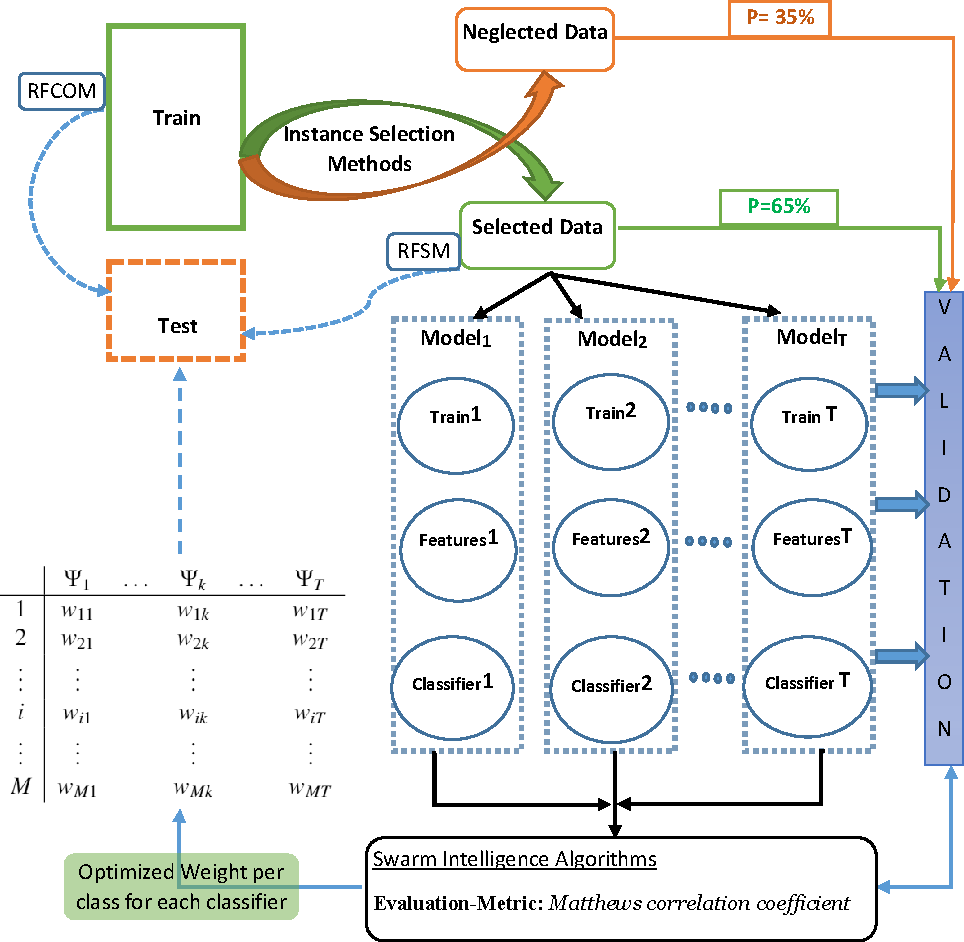
\includegraphics[width=.9\linewidth]{4_Taxonomy/figures/fig-topology.pdf}
	\caption{The proposed framework for building MCS from reduced training set.}
	\label{ch4_topology}
\end{figure}





Two models will be trained for comparison: RFSM, which denotes random forest that is trained with AllKNN-selected data, and RFCOM, which denotes random forest that is trained on the original training data. The objective is to analyze the performance of the proposed MCS against those of RFSM, RFCOM, and the following combination methods of the built classifiers:


\begin{itemize}[nosep]
	\item[-] Maj: Majority voting of the built classifiers.
	\item[-] Belief: As discussed in Section \ref{sec:4_3_beliefmethod}.
	\item[-] CW-NN: A neural network will be used to optimize class-specific weights.
	\item[-] Stacking: A neural network will be used as a  meta-classifier to tune the classifiers' weights.
\end{itemize}


\subsection{Training Set Selection} \label{Training-set-selection}
AllKNN \cite{tomek1976} removes noisy border points to produce a smoother decision boundary. The reduction capacity of this algorithm is not high, but acceptable prediction accuracy is realized over the test data. For $i=1$ to $K$ neighbors, flag as incorrect any instance that is not classified correctly by its $i$ nearest neighbors. After completing the loop, all instances that have been flagged as bad are removed \cite{alcala2011}. This method performs well if the classes are represented sufficiently well. Otherwise, the total disappearance of minor classes can be induced. This method depends on $K$ neighbors and the distance function. The default setup of $K=3$ with the Euclidean distance has been used.

AllKNN is selected as the instance selection method because it reasonably balances the reduction rate, the accuracy of the resulting model, and the execution time; as demonstrated in \cite{garcia2011}.


\subsection{Proposed MCS}\label{proposed.mcs}

MCS will be built from the selected data with the following characteristics:
\begin{itemize}[nosep]
	\item Samples diversity: Bagging is used to obtain various training samples for each individual classifier.
	\item Feature space diversity: Sixty percent of the features are selected randomly for each classifier. This procedure is repeated 20 times before selecting the most diversified set with the highest Hamming distance over the selected sub-features.
	\item Learning model diversity: Five types of classification models, namely, \textit{DT}\footnote{Package C50 :https://cran.r-project.org/web/packages/C50/index.html}, \textit{NB}\footnote{Package e1071:https://cran.r-project.org/web/packages/e1071/index.html}, \textit{JRip}\footnote{Package RWeka:https://cran.r-project.org/web/packages/RWeka/index.html}, \textit{Multinom}\footnote{Package nnet:http://cran.r-project.org/web/packages/nnet/index.html} and \textit{KNN}\footnote{Package caret:https://cran.r-project.org/web/packages/caret/index.html} are used with a proportional representation of 20\% by each model from the whole pool size. Those models are described in Section \ref{sec:2_2_SML}.
\end{itemize}




\subsection{Proposed Candidate Solution}
The power of SI relies upon stochastic operators \cite{bianchi2009,hassanien2018}, information sharing, and the preservation of search space information throughout the iterations \cite{mirjalili2016}. SI algorithms will be used to improve the fusion of MCS by optimizing the decision weight of each classifier based on its class prediction. Each candidate solution ($X$) from the population of search agents simulates the same representation schema, as expressed in Equation (\ref{CSW}). Thus, each solution represents practical weights to be used for multiple-decision fusion. All weights $w_{ik}$ are restricted to be in [0,1] $\forall i \in \{1, 2, \dots, M\}$, $\forall k \in \{1, 2, \dots, T\}$
\begin{gather}
	\label{CSW}
	\begin{array}{c|ccccc}
		       & \Psi_1 & \dots & \Psi_k  & \dots & \Psi_T  \\ \hline
		1      & w_{11} &       & w_{1k}  &       & w_{1T}  \\
		2      & w_{21} &       & w_{2k}  &       & w_{2T}  \\
		\vdots & \vdots &       & \vdots  &       & \vdots  \\
		i      & w_{i1} &       & w_{ik}  &       & w_{iT}  \\
		\vdots & \vdots &       & \vdots  &       & \vdots  \\
		M      & w_{M1} &       & w_{M k} &       & w_{M T}
	\end{array}
\end{gather}


\subsection{Proposed Objective Function} \label{Mcc-objective}
The accuracy of the proposed MCS is optimized according to the MCC metric \cite{matthews1975}. MCC is a correlation coefficient between the target and the prediction. It is always in the interval [-1,1], where +1 corresponds to a completely correct prediction. MCC realizes a good satisfactory compromise among
discrimination capability, consistency, and coherent behavior in binary and multiclass problems \cite{jurman2012}. Each candidate solution ($X$) from the social flock represents a potential set of weight coefficients that should be tuned to maximize MCC(\textit{pred($X$), target}); Equation (\ref{eq.mcc}). Where, \textit{pred($X$)} is  the ensemble prediction over the validation set using fusion weights of $X$, and is calculated via Equation (\ref{eq.objective}). While \textit{ target} is the real class column from the validation set.

\begin{equation}
	\label{eq.mcc}
	MCC=\frac{TP\times TN - FP\times FN}{\sqrt{(TP +FP)(TP+FN)(TN+FP)(TN+FN)}}
\end{equation}

\begin{equation}
	\label{eq.objective}
	pred(X)=\hat{\Psi}(\textbf{x})=\mathop{\arg\max}\limits_{i \in {M}} \mathop{\sum}\limits_{k=1}^T \left[\Psi_k(\textbf{x})=i\right]w_{ik}
\end{equation}



\subsection{Moth-Flame Optimization Algorithm}\label{Sec:4_3_5-MFO}
The MFO algorithm, which was proposed in \cite{mirjalili2015a}, was inspired by the navigation method of moths during the night. Moths use transverse orientation for navigation according to the moonlight, but their movement is affected by artificial human lights, which cause deadly spiral paths. This algorithm mimics the death behavior of moths that is caused by following artificial lights. Consider a feasible search space  $S=\{X_1, X_2,...., X_N\}$ that contains a set of positions for $N$ moths. Each moth position ($X_i$) represents the potential fusion weights for aggregating a set of classifiers. The promising areas that are identified during the search process are flagged or pinned as lights (flames); therefore, other moths can follow those lights to search for food. Hence, the initial fusion weights will be tuned by searching around promising weights iteratively.

Due to the intelligent mimic, it is possible to discover the global and local regions in the search space by simulating the spiral path of a moth around a flame via Equation (\ref{spiralmoth}). The new position of the moth will be on a hyper ellipse around the flame with a random number $\hat{t} \in$ $[r,1]$, where $r$ is linearly decreased from -1 to -2 throughout the iterations. While $D_i$ is the distance between the moth ($X_i$) and the flame ($F_j$), which is calculated via Equation (\ref{distancemoth}) and $b$ is a constant for defining the shape of the logarithmic spiral, it takes +1 in the open-source code.

\begin{equation}\label{spiralmoth}
	S(X_i,F_j)= {D_i} \cdot e^{b\hat{t}} \cdot cos\Big(2\pi\cdot \hat{t} \Big) + F_j
\end{equation}

\begin{equation}\label{distancemoth}
	{D_i}= |F_j - X_i|
\end{equation}


The flame matrix collects the best fusion weights for each moth during the search process. Consequently, it is useful for retaining the previous best solutions, and it will specify the lights where other moths can fly around to find more promising weights. The flame matrix is updated by considering both the current population and the past population of moths, which are denoted as $P_t$ and $P_{t-1}$, respectively. The best weights from the past and the current iterations are sorted in descending order to serve as the source for updating the current moth positions in the next iteration via Equation (\ref{spiralmoth}). To reduce the stochastic process in the final iterations, a focus on the exploitation milestone is realized by reducing the number of flames throughout the iterations via Equation (\ref{red-flame}).

\begin{equation}\label{red-flame}
	N{\_}{flames}= round\left(N-t *\frac{N-1}{t_{max}} \right)
\end{equation}
where $N,$ $t,$ and $t_{max}$ represent the maximum flame size, the current iteration number, and the maximum number of iterations, respectively. Via this methodology, only the best flame, which corresponds to the best-obtained fusion weight, will remain at the final iteration to guide all other moths. The pseudocode of MFO is presented in Algorithm \ref{MFO}.

\begin{algorithm}
	\caption{The pseudocode of MFO algorithm. \label{MFO}}
	\SetKwFunction{fitness}{$f$}
	\SetKwInOut{Input}{Input}
	\SetKwInOut{Output}{Output}
	\Input{Population $P=\{X_1,X_2,....,X_N\}$, Parameters ({$r, \hat{t}$, $N\_flames$}), decisions of classifiers over validation set, real class column from validation (target).}
	\Output{$X^*$ {\textit{ \quad  /* Optimized set of weight coefficients}} }

	\Begin{

	$\text{\textit{Calculate Fitness}: Mcc(pred($X_i$),target)}, i\in\{1,2,3,...,N\}  \text{ via Eq. (\ref{eq.mcc})}$\;
	\For{$t\leftarrow 1$ \KwTo $(t_{max}-1)$}{

	$\text{Update number of flames}\;
		\text{via Eq. }(\ref{red-flame})$\;


	\uIf{$\textit{iteration} == 1$} {
		$\text{Flames= sort(P)}$\;
	}
	\uElseIf{$\textit{iteration} > 1$}{
	$\text{Flames=sort($P_{t-1},P_{t}$)}$\;
	}

	$\text{Update r and \^{t}}$\;
	$\text{Calculate $D$}\;   \text{via Eq.  }(\ref{distancemoth})\; \text{for each Moth} $\;
	$\text{Update Moth position via}\; \text{ Eq. }(\ref{spiralmoth})  $\;
	$\text{Calculate fitness for each updated Moth}$\;
	}
	$\text{Return } X^*$\;
	}
\end{algorithm}


\subsection{Grey Wolf Optimizer }\label{GWOalgo}
GWO, which was proposed in \cite{mirjalili2014}, is inspired by the hierarchal leadership and hunting mechanism of grey wolves against prey. Grey wolves follow a strictly dominant social hierarchy. The most powerful wolf is $\alpha$ which is responsible for making decisions about hunting, sleeping place, and migration. The $\beta$ wolves are members in the second level that obey the alpha's decisions and give commands to the $\delta$ wolves. The $\delta$ wolves include scouts, sentinels, elders, hunters, and caretakers. The $\omega$ wolves are the lowest-ranking wolves in the group and play the role of scapegoat when there is no food.
Let $S\subset R^n$ be the feasible search space, where $S=\{X_1, X_2,...., X_N\}$ contains the set of positions for $N$ grey wolves. Each solution ($X_i$) represents possible fusion weights for the aggregation of a set of classifiers. The best grey wolves ($\alpha,\beta,\delta$) provide suitable estimates of the location of the prey (suitable fusion weights) and guide the other $\omega$ wolves in tracking and chasing the prey. Before attacking, the $\omega$ wolves encircle and harass the prey until it stops moving according to Eq. (\ref{update}).

\begin{equation}
	\label{update}
	\begin{aligned}
		X_1 & =X_\alpha(t)-A_{1} \cdot D_\alpha & \quad D_\alpha=|C_1 \cdot X_\alpha-X(t)| \\
		X_2 & =X_\beta(t)-A_{2} \cdot D_\beta   & \quad D_\beta=|C_2 \cdot X_\beta-X(t)|   \\
		X_3 & =X_\delta(t)-A_{3} \cdot D_\delta & \quad D_\delta=|C_3 \cdot X_\delta-X(t)|
	\end{aligned}
\end{equation}

\noindent where $X(t)$ is the fusion weights to be enhanced by each $\omega$ wolf. The controlling vectors $A$ and $C$ balance exploration and exploitation via Equation (\ref{parameters}) with $r_1$ and $r_2$ as random vectors $\in$ [0,1]. $C$ returns a random value in the interval $[0,2]$. The effect of gravity on the prey is increased when $C>1$.  The value of $A$ is defined by the parameter $a$, which is linearly decreased from 2 to 0 throughout the iterations. The range of $A$ is always in the interval $[-2,2]$. Exploration is promoted in the first half of the iterations when $A > 1$ or $A < -1$, whereas exploitation is forced in the second half of the iterations when $-1 < A < 1$.

\begin{equation}
	\label{parameters}
	\begin{aligned}
		C = 2 \cdot r_2      \\
		A = 2a \cdot r_1 - a \\
		a = 2 - t(\frac{2}{t_{max}})
	\end{aligned}
\end{equation}

Unsuitable fusion weights, $\omega$ wolves, will be tuned by chasing and searching around the proper fusion weights that are estimated by $\alpha$, $\beta$, and $\delta$ wolves using Equation (\ref{allthree}).
\begin{equation}
	\label{allthree}
	X(t+1)=\frac{X_1+X_2+X_3}{3}
\end{equation}

\noindent Where $X_1$, $X_2$, and  $X_3 $ are calculated as in Equation (\ref{update}). According to the discussion above, GWO depends on very few parameters ($a, A,$ and $C$) that are updated prior to position updating. The pseudocode of GWO  is presented in Algorithm \ref{GWO}.



\begin{algorithm}[!ht]
	\caption{The pseudocode of GWO algorithm. \label{GWO}}
	\SetKwFunction{fitness}{$f$}
	\SetKwInOut{Input}{Input}
	\SetKwInOut{Output}{Output}
	\Input{ Population $P=\{X_1,X_2,....,X_N\}$, Parameters ({$a, A, C$}), decisions of classifiers over validation set, real class column from validation (target).}
	\Output{$X_{\alpha}$  {\textit{ \quad  /* Optimized set of weight coefficients}} }


	\Begin{
		$\text{\textit{Calculate Fitness}: Mcc(pred($X_i$),target)}, i\in\{1,2,3,...,N\} \text{ via Eq. (\ref{eq.mcc})}$\;

		$X_\alpha \leftarrow  \text{The best search agent} $\;
		$X_\beta \leftarrow  \text{The second best search agent}
		$\;
		$X_\delta \leftarrow  \text{The third best search agent} $\;
		\For{$t\leftarrow 1$ \KwTo $(t_{max}-1)$}{
			$\text{Update position}\; \forall \omega \; \text{via Eq. }(\ref{update},\ref{allthree})$\;
			$\text{Update}\; a,$ $A,$ and $ C \; \text{via Eq. }(\ref{parameters})$\;
			$\text{Calculate fitness for each updated wolf}$\;
			$\text{Update}\; X_\alpha,X_\beta, X_\delta$\;
		}
		$\text{Return } X_\alpha$\;
	}
\end{algorithm}




\subsection{Whale Optimization Algorithm } \label{Sec:4_3_5-WOA}

This algorithm was originally developed in \cite{mirjalili2016} for mimicking the hunting behaviors of humpback whales. These whales are intelligent creatures that can sense and learn. The mathematical model simulates the feeding of humpback whales on krill and small fish herds by creating a bubble in a spiral shape around them. The optimization algorithm is similar to the GWO for encircling the prey, as described in Section \ref{GWOalgo}. The power of this algorithm is derived from its focus on fewer stochastic operators and its balancing between exploration and exploitation. Suppose $S=\{X_1, X_2,...., X_N\}$ is the feasible search space with a set of positions for $N$ whales. Each whale ($X_i$) represents a prospective fusion weights for the aggregation of a set of classifiers. During the first half of the iterations, each whale $X_i$ is forced to discover search regions by selecting a whale randomly and moving away from its location according to Equation (\ref{exploration}).

\begin{equation}
	\label{exploration}
	\begin{aligned}
		X_i(t+1) & =X_{rand}- A \cdot D      \\
		D        & =|C\cdot X_{rand}-X_i(t)|
	\end{aligned}
\end{equation}




\noindent where $A$ and $C$ are coefficient vectors having the same effect and values as calculated by Equation (\ref{parameters}). Exploration is promoted in the first half of the iterations when $A > 1$ or $A < -1$, whereas exploitation is forced in the second half of the iterations when $-1 < A < 1$.


During the second half of the iterations, the other whales $X_i$ adapt their location by encircling $X^*$ (suitable fusion weights) via Equation (\ref{whalecircle}) or by updating their spiral positions via Equation (\ref{spiral}), based on a random parameter $p$.

\begin{equation}
	\label{whalecircle}
	\begin{aligned}
		X_i(t+1) & =X^*(t)-A \cdot D       \\
		D        & =|C\cdot X^*(t)-X_i(t)|
	\end{aligned}
\end{equation}


\begin{equation}\label{spiral}
	\begin{aligned}
		X_i(t+1) & = {D}' \cdot e^{b\ell} \cdot cos(2\pi \ell) + X^*(t) \\
		{D}'     & = | X^*(t)-X_i(t)|
	\end{aligned}
\end{equation}

\setlength\intextsep{0mm}

\begin{algorithm}[!ht]
	\caption{The pseudocode of WOA algorithm. \label{WOA}}
	\SetKwFunction{fitness}{$f$}
	\SetKwInOut{Input}{Input}
	\SetKwInOut{Output}{Output}
	\Input{ Population $P=\{X_1,X_2,....,X_N\}$, Parameters ({$a, A, C, \ell$, \textit{ p}}), decisions of classifiers over validation set, real class column from validation (target).}
	\Output{$X^*$  {\textit{ \quad  /* Potential set of weight coefficients}} }



	\Begin{
		$\text{Initialize $a, A, C, \ell$, $p$ }  $\;
		$\text{\textit{Calculate Fitness}: Mcc(pred($X_i$),target)}, i\in\{1,2,3,...,N\} \text{ via Eq. (\ref{eq.mcc})}$\;
		$X^*=$  $\text{The best search agent}$\;
		\For{$t\leftarrow 1$ \KwTo $(t_{max}-1)$}{
			\uIf{$\mid A\mid \geqslant$ 1} {
				$\text{Select random search agent $X_{rand}$}$\;
				$\text{Update position of}\;  X_i \; \text{via Eq. }(\ref{exploration})$\;
			}
			\uElseIf{$\mid A\mid < $ 1}{
				\uIf{$\textit{p} < 0.5$}{
					$\text{Update position of}\;  X_i \; \text{via Eq. }(\ref{whalecircle})$\;
				}
				\uElseIf{$\textit{p} \geqslant 0.5$}{
					$\text{Update position of}\;  X_i \; \text{via Eq. }(\ref{spiral})$\;}
			}

			$\text{Calculate the fitness of each search agent}$\;
			$\text{Update $X^*$  if there is better solution}  $\;
			$\text{Update Parameters ($a, A, C, \ell$, $p$)} $\;
		}
		$\text{Return } X^*$\;
	}
\end{algorithm}

As a result, the local search and the exploitation process can be enhanced. ${D}'$ represents the distance between two whales, $b$ is a constant for defining the shape of the logarithmic spiral and $\ell$ is a random number in [-1,1].  The pseudocode of WOA is presented in Algorithm \ref{WOA}. \textit{The implementations of the SI algorithms that have been used in this chapter are from R package}: metaheuristicOpt. \footnote{SI:https://cran.r-project.org/web/packages/metaheuristicOpt/index.html}

